\documentclass[11pt]{article}
\usepackage[T1]{fontenc}
\usepackage[utf8]{inputenc}
\usepackage[a4paper,margin=27mm]{geometry}
\usepackage{amsmath,amssymb,amsthm,mathtools,booktabs,array}
\usepackage{tikz}
\usetikzlibrary{arrows.meta,calc,positioning,decorations.pathreplacing}
\usepackage[hidelinks]{hyperref}
\usepackage{xurl}
\newtheorem{theorem}{Theorem}[section]
\newtheorem{lemma}[theorem]{Lemma}
\newtheorem{proposition}[theorem]{Proposition}
\newtheorem{corollary}[theorem]{Corollary}
\newcommand{\HH}{\mathbb H}
\newcommand{\ip}[2]{\langle #1,#2\rangle}
\newcommand{\Pthree}{P_3}
\newcommand{\Qeight}{Q_8}
\newcommand{\EE}{\mathbb E}
\newcommand{\file}{\path}
\tikzset{finite/.style={circle,draw,fill=black,inner sep=2.1pt},
 ideal/.style={circle,draw,fill=white,inner sep=2.7pt},
 every picture/.style={line cap=round,line join=round},
 move/.style={-{Stealth[length=2mm]},thick,blue!65!black}}
\title{A dimension bound of eleven for right-angled hyperbolic polytopes}
\author{Coxeter Polytopes Frontier Project}
\date{19 October 2026; internal research manuscript}
\begin{document}
\maketitle
\begin{abstract}
We exclude finite-volume right-angled hyperbolic polytopes with both
finite and ideal vertices in dimension twelve. A canonical
three-face defines an undirected opposition graph on the finite
vertices. Its invariant Lorentz vector allows one fixed null direction
on each component. Exact subset moments and a positive-part quartic
majorant give $2B\le(1420561/12500)f$, where $B$ counts these
three-faces and $f$ counts finite vertices. Polygon incidences and an
exception budget for three-faces give the incompatible strict lower
bound $2B>(184460/1619)f$. Together with the published higher-dimensional
exclusion, the mixed dimension bound is eleven. The compact and entirely
ideal cases have smaller published bounds, so eleven also bounds all
finite-volume right-angled polytopes. The geometric and scalar arguments
are given in full. A small exact coefficient certificate and conditional
Lean checks of the final counting logic are separate verification layers;
the geometry is not fully formalized, and no new example or sharpness
claim is made.
\end{abstract}

\section{Statement, conventions and external inputs}
\begin{theorem}\label{thm:main}
A finite-volume right-angled hyperbolic polytope having both finite
and ideal vertices has dimension at most eleven.
\end{theorem}
\begin{corollary}\label{cor:all}
Every finite-volume right-angled hyperbolic polytope has dimension
at most eleven.
\end{corollary}
We use Dufour's published bound twelve~\cite{Dufour} to reduce
Theorem~\ref{thm:main} to dimension twelve. The compact and entirely
ideal bounds four and six~\cite{PV,Kolpakov} then give
Corollary~\ref{cor:all}. These previous bounds are theorem inputs,
not conclusions of the new opposition argument. Examples in dimension
eight do not establish sharpness of the new upper bound.

Until the final contradiction let $P\subset\HH^{12}$ be a hypothetical
mixed right-angled polytope. Write $f>0$ for its finite vertices,
$c>0$ for its ideal vertices, and $a_j$ for its $j$-faces. The
letter $B$ will count a specific three-face defined below; it never
denotes the number of triangular polygons or all three-faces.

Use Lorentz signature $(12,1)$, future unit timelike representatives
$q^2=-1$ for finite points, and outward unit spacelike normals $r$.
Wall inequalities are $\ip{x}{r}\le0$. Distinct outward normals
have nonpositive products. At a finite vertex $q$, the twelve incident
normals $n_1,\ldots,n_{12}$ are orthonormal; direction $i$ is the edge
obtained by omitting $n_i$. Ideal vertices are future null rays.
Faces of dimension at least three inherit finite volume and right
angles. Two-faces are hyperbolic polygons with finite angles $\pi/2$
and ideal angles zero.

The external structural inputs are these standard acute-wall/link facts,
simple truncation at ideal vertices and Dehn--Sommerville symmetry, and
the published lower bound of $82$ for the number of facets of a finite-volume
right-angled eight-polytope. The last bound and the truncation conventions
are recorded in Alexandrov's Sections 2--6~\cite{Alex}. The absence of
compact right-angled polytopes above dimension four ensures that this
noncompact lower bound applies to every eight-face used below.
All small-three-face geometry, moment calculations, scalar inequalities
and incidence eliminations needed for the new exclusion are proved here.
No restriction on a facet spectrum or arithmetic field is imposed.

\section{Actual three-face oppositions}
\subsection{Projection and the normal-product gap}
\begin{lemma}\label{lem:gap}
Two distinct unit outward facet normals of a right-angled polytope
have scalar product zero or at most $-1$.
\end{lemma}
\begin{proof}
Acuteness gives a product $g\le0$. Suppose $-1<g<0$. Their
Gram matrix $G=\left(\begin{smallmatrix}1&g\\g&1\end{smallmatrix}\right)$
is positive definite and $G^{-1}$ is entrywise nonnegative. For a
strict future timelike interior point $x$, put
$b=(\ip{x}{u},\ip{x}{v})^T<0$ and
$x_0=x-[u\ v]G^{-1}b$. The coefficients added to $x$ are positive,
so every other wall $r$ satisfies
$\ip{x_0}{r}\le\ip{x}{r}<0$. Moreover
$x_0^2=x^2-b^TG^{-1}b<0$ and $\ip{x_0}{x}<0$.
Thus $x_0$ is a relative-interior point of an actual ridge with a
nonright angle, a contradiction.
\end{proof}
The same argument with an orthonormal root set proves actual
feasibility of its projected intersection. Positive null sums of
actual outward normals are also useful: acuteness checks every other
wall, and strict interior pairing proves such a sum is nonzero and
future. It therefore represents a feasible ideal point.

Call a two-face with one finite and two ideal vertices a
\emph{bad triangle}; the name denotes a counted type, not a forbidden
face. At a finite $q$, form a graph $G_q$ on the twelve directions,
with $ij$ an edge when their two-face is a bad triangle.
Its two ideal endpoints are $q-n_i,q-n_j$. The opposite wall has
the uniquely oriented unit normal
\begin{equation}\label{eq:badwall}
 m_{ij}=q-n_i-n_j.
\end{equation}
This follows by orthogonality to the other incident normals, incidence
with the two endpoints and unit norm; the displayed sign is strict
at $q$.

\begin{lemma}\label{lem:P3}
Each triangle $S=\{i,j,k\}$ in $G_q$ determines an actual three-face
$\Pthree$, the triangular bipyramid with two finite vertices and three
ideal vertices. Its other finite vertex is
\begin{equation}\label{eq:opposite}
 q_S=2q-n_i-n_j-n_k.
\end{equation}
Its six polygon facets are bad triangles.
\end{lemma}
\begin{proof}
The three actual normals $m_{ij},m_{ik},m_{jk}$ are orthonormal.
The displayed $q_S$ has square $-1$ and $\ip{q}{q_S}=-2$, so
is future timelike. It vanishes on these three walls and on the
$n_l$ outside $S$. The old $n_i,n_j,n_k$ have strictly negative
products there.

To check all remaining walls, write their unit normals in the complete
$q,n_l$ frame as $r=a q-\sum_l c_l n_l$. Strictness at $q$ gives
$a>0$ and acuteness gives $c_l\ge0$. For $r$ distinct from the
three selected $m$ walls, their acute products imply
\[
 c_i+c_j\le a,\qquad c_i+c_k\le a,\qquad c_j+c_k\le a.
\]
Consequently $\ip{r}{q_S}=-2a+c_i+c_j+c_k\le-a/2<0$.
Thus $q_S$ is an actual simple finite vertex with exactly the
specified incident walls.

In the Lorentz four-space spanned by $q,n_i,n_j,n_k$, the six
known inequalities are, for $x=tq-\sum y_l n_l$,
$y_l\ge0$ and $y_l+y_m\le t$. They enclose precisely the
finite-volume convex hull of $q,q_S,q-n_i,q-n_j,q-n_k$.
All five points belong to $P$. Convexity therefore prevents any
additional wall from cutting this hull; the three-face is exactly
that bipyramid. Its six facets have the asserted vertex types.
\end{proof}

\begin{figure}[ht]
\centering
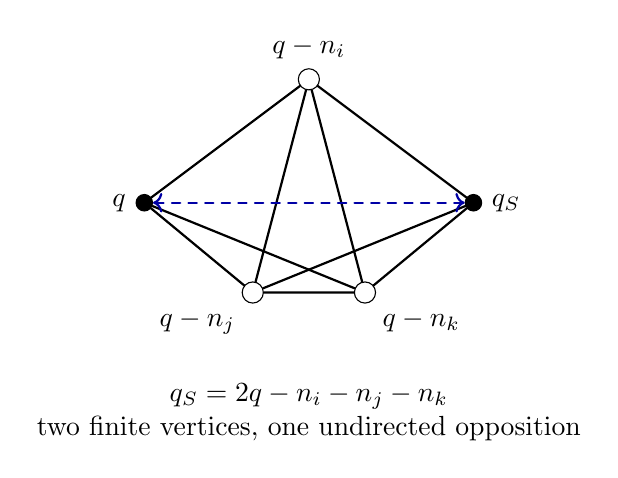
\begin{tikzpicture}[scale=.95]
 \node[finite,label=left:{$q$}] (q) at(-2.2,0){};
 \node[finite,label=right:{$q_S$}] (p) at(2.2,0){};
 \node[ideal,label=above:{$q-n_i$}] (i) at(0,1.65){};
 \node[ideal,label=below left:{$q-n_j$}] (j) at(-.75,-1.2){};
 \node[ideal,label=below right:{$q-n_k$}] (k) at(.75,-1.2){};
 \draw[thick] (i)--(j)--(k)--(i);
 \foreach \v in {i,j,k}{\draw[thick] (q)--(\v) (p)--(\v);}
 \draw[blue!65!black,thick,dashed,<->] (q)--(p);
 \node[align=center] at(0,-2.8)
 {$q_S=2q-n_i-n_j-n_k$\\two finite vertices, one undirected opposition};
\end{tikzpicture}
\caption{The actual $\Pthree$ three-face. This is an incidence drawing,
not a metric projection. Hollow vertices are ideal. The dashed
opposition segment is not an edge of the polytope.}
\label{fig:P3}
\end{figure}

Let $B$ count all three-faces isometric to $\Pthree$. Every such
face gives one triangle of $G_q$ at each of its two finite vertices,
and Lemma~\ref{lem:P3} gives the converse. Different triples at $q$
give different opposites, by linear independence of the $n_i$.
Thus they form a finite undirected graph on all finite vertices,
with exactly $B$ edges and degree sum $2B$.

\subsection{A fixed null direction on each opposition component}
\begin{lemma}\label{lem:invariant}
The vector $h=3q-\sum_{i=1}^{12}n_i$ is constant across every
actual opposition edge. It has $h^2=3$ and $\ip{h}{q}=-3$.
On each opposition component one can fix a nonzero future null
vector $Z$ with $\ip{Z}{h}=0$.
\end{lemma}
\begin{proof}
At $q_S$ the new three normals are the $m$ in
\eqref{eq:badwall}; the other nine normals are unchanged. Their
total is $3q+\sum_i n_i-3\sum_{i\in S}n_i$. Substitution in
$3q_S$ minus this sum gives exactly $h$. The stated square and
product follow from the orthonormal frame. Since $h$ is spacelike,
its orthogonal complement is Lorentzian and contains a future null
direction. Choose one on each component, including isolated vertices.
The choice does not require complete corner graphs.
\end{proof}
Put
\begin{equation}\label{eq:normalization}
 E(q)=-\ip{Z}{q}>0,\qquad
 p_i=-\frac{\ip{Z}{n_i}}{E(q)},\qquad g(q)=E(q)^{-2}.
\end{equation}
The same $Z$ is used at both endpoints of every actual edge.
Componentwise rescaling of $Z$ cancels from all edge ratios.
Decomposition $Z=E(q)(q-\sum p_i n_i)$, together with $Z^2=0$
and $\ip{Z}{h}=0$, gives
\begin{equation}\label{eq:p}
 \sum_i p_i=3,\qquad \sum_i p_i^2=1.
\end{equation}
There is no assumption that individual $p_i$ are nonnegative.

\section{Formal triples and their exact moments}
Set $x_i=p_i-1/4$. Then $\sum x_i=0$ and $\sum x_i^2=1/4$.
For \emph{all} $220$ three-subsets $S$ define the formal vector
$q_S=2q-\sum_{i\in S}n_i$, whether or not it is an actual
opposition. It is future unit timelike, since $q_S^2=-1$ and
$\ip{q}{q_S}=-2$. Its formal energy ratio is therefore positive:
\begin{equation}\label{eq:r}
 r_S=\frac{E(q_S)}{E(q)}=2-\sum_{i\in S}p_i
     =\frac54+d_S,\qquad d_S=-\sum_{i\in S}x_i.
\end{equation}
The centered indicator of a three-subset has squared norm $9/4$.
Cauchy--Schwarz gives $|d_S|\le3/4$, hence
\begin{equation}\label{eq:domain}
 \frac12\le r_S\le2.
\end{equation}
No formal vector is presumed to be a feasible chamber vertex.

\begin{lemma}\label{lem:moments}
Uniform averages over the $220$ formal triples at a fixed finite vertex
satisfy
\begin{align*}
 \EE d&=0,&\EE d^2&=\frac9{176},\\
 \EE d^3&=-\frac{27}{220}\sum_i x_i^3,&
 \EE d^4&=\frac3{440}-\frac3{220}\sum_i x_i^4\le\frac3{440}.
\end{align*}
Moreover $-\EE d^3\le27/1760$.
\end{lemma}
\begin{proof}
The inclusion probabilities for one, two and three specified indices
are respectively $1/4,1/22,1/220$. With $s_j=\sum_i x_i^j$ and
$s_1=0$, the second moment is $(1/4-1/22)s_2=9/176$.
The coefficient of $s_3$ in the third subset-sum moment is
$1/4-3/22+2/220=27/220$; the sign reverses for $d$.
The fourth expansion is
\[
 (1/4-7/22+12/220)s_4+(3/22-6/220)s_2^2
 =-3s_4/220+3/440.
\]
Finally $|s_3|\le\sum|x_i|^3\le s_2^{3/2}=1/8$.
\end{proof}

\section{A positive-part quartic bound}
The pointwise scalar inequality needed for deletion of absent formal
triples is stronger than a reciprocal estimate alone.
\begin{lemma}\label{lem:quartic}
For $-3/4\le d\le3/4$, put
\[
 P(d)=\frac{19}{125}-\frac{979}{1000}d
      +\frac{768}{625}d^2-\frac{971}{3125}d^3
      +\frac{53186}{9375}d^4.
\]
Then
\begin{equation}\label{eq:majorant}
 P(d)\ge\max\left\{0,\left(\frac54+d\right)^{-2}-\frac12\right\}.
\end{equation}
\end{lemma}
\begin{proof}
We prove nonnegativity and reciprocal majorization separately.
For $d\le0$ every term of $P$ is nonnegative. For $d\ge0$,
\[
 P''(d)-\frac{12}5
 =\frac{36}{625}-\frac{5826}{3125}d+\frac{212744}{3125}d^2
 \ge\frac{36}{625}-2d+60d^2>0.
\]
The last quadratic has minimum $36/625-1/60>0$. At $d_0=1/4$,
\[
 P(d_0)=\frac{1627}{1200000}>\frac{13}{10000},\qquad
 P'(d_0)=-\frac{10243}{150000},\quad |P'(d_0)|<\frac7{100}.
\]
The strong-convexity lower parabola gives
\[
 P(d)\ge\frac{13}{10000}-\frac{(7/100)^2}{24/5}
       =\frac{67}{240000}>0\qquad(d\ge0).
\]

Write $r=\mu+d$, $\mu=5/4$. The exact reciprocal-square identity is
\begin{equation}\label{eq:reciprocal}
 r^{-2}=\mu^{-2}-2d\mu^{-3}+3d^2\mu^{-4}-4d^3\mu^{-5}
          +\frac{d^4(4r+\mu)}{\mu^5r^2}.
\end{equation}
It follows by multiplying by $\mu^5r^2$ and expanding. Since
$(4r+\mu)/r^2$ decreases for $r>0$, its maximum for $r\ge1/2$
is $13$. Thus $r^{-2}-1/2$ is at most
\[
 P_0(d)=\frac7{50}-\frac{128}{125}d+\frac{768}{625}d^2
       -\frac{4096}{3125}d^3+\frac{13312}{3125}d^4.
\]
For $d\ge0$ the difference
\[
 P-P_0=\frac3{250}+\frac9{200}d+d^3+\frac{106}{75}d^4
\]
is nonnegative. This proves reciprocal majorization on that half.

For $d=-t$, $0\le t\le3/4$, direct multiplication gives
\begin{align}
 N(t)&=\left(\frac54-t\right)^2
       \left(P(-t)-\left(\frac54-t\right)^{-2}+\frac12\right)
       \notag\\
 &=\frac3{160}-\frac{321}{3200}t+\frac{249}{2000}t^2
   -\frac{643}{400}t^3+\frac{27949}{3000}t^4
   -\frac{130052}{9375}t^5+\frac{53186}{9375}t^6.
 \label{eq:N}
\end{align}
We give a rational certificate that $N>0$ on this entire interval.
For a degree-$m$ polynomial $Q$, write
$Q(a+(b-a)u)=\sum_{k=0}^m c_k u^k$ and define
\[
 \beta_i=\sum_{k=0}^i c_k\frac{\binom ik}{\binom mk}.
\]
The binomial theorem gives
$Q(a+(b-a)u)=\sum_i\beta_i\binom mi u^i(1-u)^{m-i}$.
On $0\le u\le1$ the basis is nonnegative and sums to one.
Thus bounds on these coefficients control the full interval.
Expansion of~\eqref{eq:N} gives the following strict bounds on all
successive coefficients; the displayed formula makes each a direct
rational check.
\begin{center}
\small
\begin{tabular}{p{.23\linewidth}p{.68\linewidth}}\toprule
Polynomial and interval&Bounds on successive Bernstein coefficients\\\midrule
$N'$ on $[0,1/5]$, degree $5$&
Less than $-1/10,-9/100,-99/1000,-98/1000,-79/1000,-9/200$\\[2mm]
$N'$ on $[3/10,1/2]$, degree $5$&
Greater than $3/50,11/100,17/100,21/100,23/100,1/5$\\[2mm]
$N''$ on $[1/2,3/4]$, degree $4$&
Less than $-3/5,-19/10,-37/10,-29/5,-36/5$\\\bottomrule
\end{tabular}
\end{center}
The first row makes $N$ decreasing on $[0,1/5]$, where
$N(1/5)>1/1000$ proves positivity.

On the central interval $[1/5,3/10]$, the quadratic $N''''$ is
convex and has endpoint values less than $-27,-91$, so it is
negative throughout. Hence $N'''$ decreases; its endpoint value
$N'''(3/10)>9/10$ makes it positive. Therefore $N''$ increases
and $N''(1/5)>4/5$ makes $N''>1/2$ throughout. The exact midpoint
values are
\[
 N(1/4)=\frac{679}{1200000}>\frac1{2000},\qquad
 N'(1/4)=\frac{3061}{600000},\quad |N'(1/4)|<\frac1{100}.
\]
Its lower parabola gives $N\ge1/2000-(1/100)^2>0$ there.
The second Bernstein row makes $N$ increasing on $[3/10,1/2]$,
so positivity propagates from the central endpoint. The third makes
$N$ concave on $[1/2,3/4]$. Its first endpoint is positive by the
preceding interval and its last is $N(3/4)=57/64000>0$.
A concave function lies above its chord. These four intervals cover
$[0,3/4]$, proving $N>0$ and hence the remaining reciprocal bound.
\end{proof}

\begin{figure}[ht]
\centering
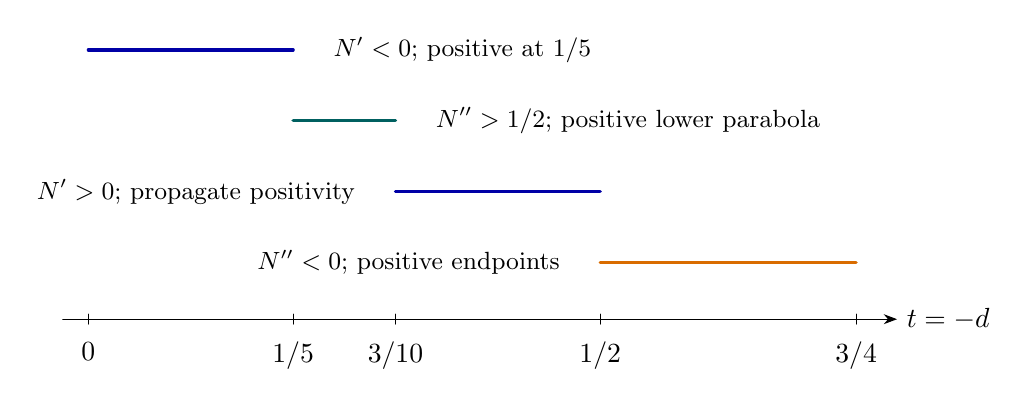
\begin{tikzpicture}[x=13cm,y=.9cm,>=Stealth]
 \draw[->](-.025,-.8)--(.79,-.8)node[right]{$t=-d$};
 \foreach \x/\lab in {0/0,.2/{1/5},.3/{3/10},.5/{1/2},.75/{3/4}}
  {\draw(\x,-.73)--(\x,-.87)node[below=3pt]{$\lab$};}
 \draw[very thick,blue!65!black](0,3)--(.2,3);
 \draw[very thick,teal!75!black](.2,2)--(.3,2);
 \draw[very thick,blue!65!black](.3,1)--(.5,1);
 \draw[very thick,orange!85!black](.5,0)--(.75,0);
 \node[anchor=west,font=\small]at(.23,3)
  {$N'<0$; positive at $1/5$};
 \node[anchor=west,font=\small]at(.33,2)
  {$N''>1/2$; positive lower parabola};
 \node[anchor=east,font=\small]at(.27,1)
  {$N'>0$; propagate positivity};
 \node[anchor=east,font=\small]at(.47,0)
  {$N''<0$; positive endpoints};
\end{tikzpicture}
\caption{The exact interval proof for $N$. The bars indicate certificate
domains, not sampled values or a plotted approximation to the polynomial.}
\label{fig:intervals}
\end{figure}

\section{Deleting absent triples and summing ordinary vertices}
\begin{proposition}\label{prop:upper}
Every finite-volume right-angled twelve-polytope satisfies
\begin{equation}\label{eq:upper}
 2B\le\frac{1420561}{12500}f.
\end{equation}
\end{proposition}
\begin{proof}
At a finite vertex let $t(q)$ be its opposition degree. For each
actual neighbor, equations~\eqref{eq:normalization}--\eqref{eq:r}
give $g(q_S)/g(q)=r_S^{-2}$. Lemma~\ref{lem:quartic} implies
\[
 r_S^{-2}-1\le P(d_S)-1/2.
\]
Sum over the actual subset of triples. Inserting the absent formal
triples on the right is legitimate because $P\ge0$, giving
\begin{equation}\label{eq:delete}
 \sum_{\text{actual }S}\left(\frac{g(q_S)}{g(q)}-1\right)
 \le\sum_{\text{all }220\ S}P(d_S)-\frac{t(q)}2.
\end{equation}
The cubic coefficient of $P$ is negative, and its quadratic and
quartic coefficients are positive. Lemma~\ref{lem:moments} therefore
gives, pointwise at every finite vertex,
\begin{align}
 \EE P&\le\frac{19}{125}
  +\frac{768}{625}\frac9{176}
  +\frac{971}{3125}\frac{27}{1760}
  +\frac{53186}{9375}\frac3{440}
  =\frac{1420561}{5500000}.\label{eq:Pmean}
\end{align}

Now sum~\eqref{eq:delete} over \emph{ordinary unweighted} finite
vertices, allowing the componentwise choices of $Z$. Each actual
undirected edge contributes a reciprocal pair
\[
 \frac{g(v)}{g(u)}+\frac{g(u)}{g(v)}-2=r^{-2}+r^2-2\ge0.
\]
Using $\sum_q t(q)=2B$ gives
$0\le220(1420561/5500000)f-B$, which is~\eqref{eq:upper}.
This summation does not select a height maximum or turn a weighted
average into an unweighted one. The constant $1/2$ is a deletion
allowance in the scalar bound, not an added move or multiplicity.
\end{proof}

\begin{figure}[ht]
\centering
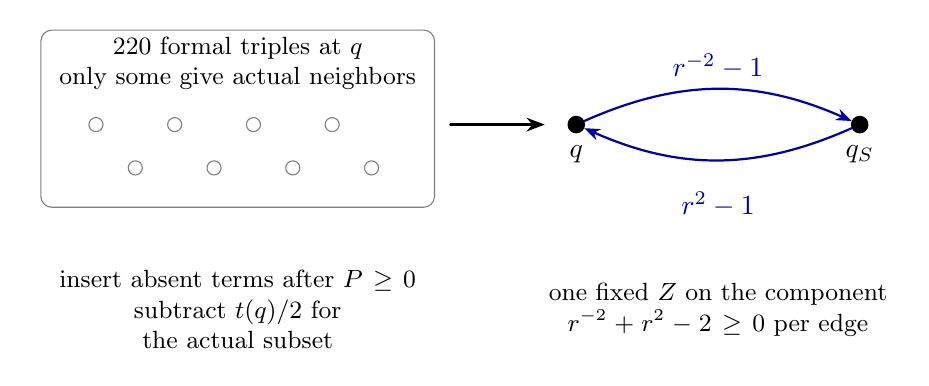
\begin{tikzpicture}[>=Stealth]
 \draw[rounded corners,gray](-5.7,-1.05)rectangle(-.7,1.2);
 \node[align=center,font=\small]at(-3.2,.78){220 formal triples at $q$\\only some give actual neighbors};
 \foreach \x/\y in {-5/0,-4.5/-.55,-4/0,-3.5/-.55,-3/0,-2.5/-.55,-2/0,-1.5/-.55}
  \node[circle,draw,gray,inner sep=1.8pt]at(\x,\y){};
 \node[finite](q)at(1.1,0){};
 \node[finite](v)at(4.7,0){};
 \node[below=4pt]at(q){$q$};\node[below=4pt]at(v){$q_S$};
 \draw[move,bend left=24](q)to node[above]{$r^{-2}-1$}(v);
 \draw[move,bend left=24](v)to node[below=8pt]{$r^2-1$}(q);
 \draw[->,thick](-.5,0)--(.7,0);
 \node[align=center,text width=5.1cm,font=\small]at(-3.2,-2.35)
 {insert absent terms after $P\ge0$\\subtract $t(q)/2$ for the actual subset};
 \node[align=center,text width=4.4cm,font=\small]at(2.9,-2.35)
 {one fixed $Z$ on the component\\$r^{-2}+r^2-2\ge0$ per edge};
\end{tikzpicture}
\caption{The actual-subset passage and reciprocal edge pairing. The
left panel is a schematic row, not a claim that every formal triple
is a chamber face. Summation on the right uses the actual graph only.}
\label{fig:pairing}
\end{figure}

\section{A strict weighted polygon row}
We next derive the opposing lower bound for the \emph{same} $B$.
At a finite vertex there are $\binom{12}{2}=66$ two-faces. At an
ideal vertex the cubical eleven-dimensional link has $11264$ edges,
so there are $11264$ two-faces. With $\lambda=2123/1280$, we need
\begin{equation}\label{eq:weighted}
 66f+11264\lambda c<\frac{22}5a_2,
 \qquad\text{equivalently }a_2>15f+4246c.
\end{equation}

Here is an explicit Dehn--Sommerville derivation. Truncate every
ideal vertex. The simple Euclidean twelve-polytope so obtained has
face counts
\[
 b_0=f+2048c,\quad b_{11}=a_{11}+c,\quad
 b_k=a_k+2^{11-k}\binom{11}{k}c\quad(1\le k\le10).
\]
In particular $b_0$ replaces each old cusp by its $2048$ link vertices;
it does not count that cusp as an additional finite vertex.
For
\[
 H(t)=(t-1)^{12}+\sum_{k=0}^{11}b_k(t-1)^k,
\]
Dehn--Sommerville gives $H(t)=t^{12}H(1/t)$. Comparing coefficients
and solving the six independent linear relations gives
\begin{align}
 f&=a_6-5a_7+14a_8-28a_9+42a_{10}-42a_{11}-462c,
 \notag\\
 a_2&=15a_6-74a_7+206a_8-411a_9+616a_{10}-616a_{11}-2684c.
 \label{eq:DS}
\end{align}
These two displayed coefficient rows can also be checked directly
by substitution into the coefficient equations for $H$; there is
no feasibility or enumeration premise. They give the identity
\begin{equation}\label{eq:weightedid}
 66f+11264\lambda c-\frac{22}5a_2
 =\frac{-22a_7+88a_8-198a_9+308a_{10}-308a_{11}}5.
\end{equation}
Every eight-face has at least $82$ facets. Since each seven-face
lies in five eight-faces, $5a_7\ge82a_8$. Similarly each
ten-polytope has at least eleven facets and each nine-face lies
in three ten-faces, so $3a_9\ge11a_{10}$. Thus
\[
 -22a_7+88a_8\le-\frac{1364}5a_8<0,\qquad
 -198a_9+308a_{10}\le-418a_{10}<0.
\]
The last term in~\eqref{eq:weightedid} is negative as well.
This proves~\eqref{eq:weighted}, with strictness.

\section{Small three-faces and an exception budget}
For a right-angled three-polyhedron write $F,s,p$ for its polygon
facets, ideal vertices and finite vertices, and put $\nu=F+s$.
Finite and ideal vertex degrees are three and four. Euler gives
\begin{equation}\label{eq:Euler3}
 p+2s=2F-4,\qquad p=4F-2\nu-4.
\end{equation}
A polygon with $u$ finite and $v$ ideal vertices has area
$\frac\pi2(u+2v-4)>0$, so the integer $u+2v-5$ is nonnegative.
Summing over the polygons yields
\begin{equation}\label{eq:excess3}
 \sum(u+2v-5)=F+2s-12\ge0.
\end{equation}
In particular $p+6s\ge20$. If $F\le5$, Euler would give
$p+2s\le6$, $s\le3$ and $p+6s\le18$, a contradiction.
Thus $F\ge6$ and $\nu\ge9$.

\begin{lemma}\label{lem:six}
Equality $F=6$ or $\nu=9$ occurs only for $\Pthree$.
\end{lemma}
\begin{proof}
At $F=6$, equation~\eqref{eq:excess3} gives $s\ge3$. There are
$24-2s$ polygon corners. At least $2s$ of the six polygons must
therefore be triangles, so $s\le3$. Hence $s=3,p=2$, and all
six facets are triangles. A positive-area right-angled triangle
has at most one finite vertex. The finite polygon-corner count
$3p=6$ then forces each triangle to have exactly one finite
vertex. At either finite vertex all three pairs are bad, and
Lemma~\ref{lem:P3} identifies the whole polyhedron. Finally
$F\ge6$ and $F+2s\ge12$ make $F+s=9$ possible only at
$F=6,s=3$.
\end{proof}

\subsection{Two triangles attached across their ideal edge}
\begin{lemma}\label{lem:attachment}
If two bad triangular facets of a right-angled three-polyhedron
share their ideal--ideal edge, the whole polyhedron is $\Pthree$.
\end{lemma}
\begin{proof}
Scale the shared future null endpoints $u,v$ so that the first
finite apex $q_1$ has products $-1$ with both. Its right angle
gives $\ip{u}{v}=-1$. Let $n_1,n_2$ be the orthogonal unit
outward normals of the two triangles. They are perpendicular to
$u,v$. The apices have the forms
\[
 q_1=u+v-n_2,\qquad q_2=t u+t^{-1}v-n_1,\quad t>0.
\]
Indeed the right angle at each apex makes the product of its two
null coefficients one; unit timelike norm then makes the normal
coefficient $\pm1$, with the negative sign fixed by orientation.
The other four actual side normals are
\[
 u-n_2,\quad v-n_2,\quad t u-n_1,\quad t^{-1}v-n_1.
\]
Two cross products are $-t,-t^{-1}$. Lemma~\ref{lem:gap}
therefore forces $t=1$. The third ideal vertex
$w=u+v-n_1-n_2$ is future null and is the sum
$(u-n_1)+(v-n_2)$ of actual outward normals. Acuteness checks
every other wall, and the selected walls also contain or accept
$w$. The six known inequalities enclose exactly the finite-volume
convex hull of $q_1,q_2,u,v,w$. All five vertices are feasible,
so convexity identifies the whole polyhedron.
\end{proof}

\subsection{The zero-excess eight-facet type}
Call a three-polyhedron with $F=8,s=2$ a $\Qeight$ type;
metric uniqueness is unnecessary. Euler gives $p=8$, and
\eqref{eq:excess3} says every polygon has zero excess. A bad
triangle would share its ideal--ideal edge with another zero-excess
polygon containing both ideal endpoints, hence another bad
triangle. Lemma~\ref{lem:attachment} would give $\Pthree$,
a contradiction. There are no triangles. Its eight polygons
have $32$ corners in total, so every one is a $(u,v)=(3,1)$
quadrilateral.

At a finite $\Qeight$ vertex there is at most one edge with
ideal other endpoint: two such directions would span a polygon
containing two ideal vertices, impossible for its quadrilaterals.
No edge joins its two cusps for the same reason. Their degree-four
links supply eight finite--ideal edges; the eight finite vertices
have at most one each, so each has exactly one.

\subsection{Every finite corner has many exceptional three-faces}
Call a three-face \emph{exceptional} when it is neither $\Pthree$
nor a $\Qeight$ type. At an ambient finite vertex $q$, let $k$
be the number of its twelve directions whose edges end at ideal
vertices, and let $t(q)$ be the number of triangles in $G_q$.
Exactly $t(q)$ of its incident three-faces are $\Pthree$.
A $\Qeight$ can use only a triple with exactly one of the $k$
ideal-ending directions, so the exceptional incidence count obeys
\[
 X(q)\ge220-t(q)-k\binom{12-k}{2}.
\]
Every bad-graph triangle uses three ideal-ending directions, hence
$t(q)\le\binom k3$. For $k=0,\ldots,12$ one has
\[
 14\left(220-\binom k3\right)-27k\binom{12-k}{2}\ge0.
\]
The complete successive integer values are
\[
 3080,1595,650,150,0,105,370,700,1000,1175,1130,770,0.
\]
It follows, with $\gamma=13/27$, that
\begin{equation}\label{eq:Xlower}
 X(q)\ge\gamma(220-t(q)),\qquad
 X:=\sum_q X(q)\ge\gamma(220f-2B).
\end{equation}
This counts actual triples and ideal edge endpoints; no
symmetrization of arbitrary corner graphs is used.

\begin{lemma}\label{lem:budget}
Every exceptional three-face satisfies
\begin{equation}\label{eq:budget}
 p\le22(\nu-10)+4(8-F).
\end{equation}
\end{lemma}
\begin{proof}
Subtracting $p=4F-2\nu-4$ from the right side gives
$24\nu-184-8F$. At $\nu=10$, equation~\eqref{eq:excess3}
gives $F\le8$. The six-facet type is $\Pthree$, and $F=8,s=2$
is $\Qeight$, both excluded. The remaining $F=7,s=3,p=4$
gives equality. At $\nu=11$, one has $F\le10$, so the
difference is $80-8F\ge0$. At $\nu\ge12$, use $F\le\nu$
to obtain $16\nu-184\ge8$. The case $\nu=9$ is only
$\Pthree$ by Lemma~\ref{lem:six}.
\end{proof}

\section{Global incidence elimination and the contradiction}
Define a nonnegative excess and a signed facet defect by
\[
 \mathcal E=\sum_{\text{non-}\Pthree}(\nu-10),\qquad
 \mathcal R=\sum_{\text{non-}\Pthree}(8-F).
\]
The second quantity need not be nonnegative and is not a face count.
Both contributions are zero for $\Qeight$, so summing
Lemma~\ref{lem:budget} over exceptional faces gives
\begin{equation}\label{eq:Xupper}
 X\le22\mathcal E+4\mathcal R.
\end{equation}
Each polygon is contained in ten three-faces. An ambient cusp
belongs to $2^9\binom{11}{2}=28160$ three-faces, by its cubical
link. Hence the exact coface identities are
\begin{equation}\label{eq:ER}
 \mathcal E=B-10a_3+10a_2+28160c,\qquad
 \mathcal R=8a_3-10a_2-2B.
\end{equation}
For example summing $\nu=F+s$ over \emph{all} three-faces gives
$10a_2+28160c$; removing the $\Pthree$ contribution to
$\nu-10$ adds $B$. Removing its $8-F=2$ contribution subtracts
$2B$ in the other identity.

We also need the finite/cusp Euler incidence identity
\begin{equation}\label{eq:a3}
 10a_2=2a_3+110f+28160c,\qquad
 a_3=5a_2-55f-14080c.
\end{equation}
To derive it, sum $F=2+p/2+s$ from~\eqref{eq:Euler3} over
all three-faces. Each finite vertex belongs to $220$ three-faces,
each cusp to $28160$, and the left side is again $10a_2$.

Combining~\eqref{eq:Xlower}--\eqref{eq:a3} gives
\begin{equation}\label{eq:coupling}
 101B-5130a_2+69080f+22049280c\ge0.
\end{equation}
For an explicit coefficient check, before substituting~\eqref{eq:a3}
and dividing by four the expression is
\[
 404B-5076a_3+4860a_2-2860f+16727040c\ge0.
\]
Using the strict weighted row~\eqref{eq:weighted} in
\eqref{eq:coupling} yields
\begin{equation}\label{eq:lowerone}
 101B>7870f-267300c.
\end{equation}

Independently, Lemma~\ref{lem:six} says $\nu\ge10$ for every
non-$\Pthree$ three-face, whereas $\Pthree$ has $\nu=9$.
Thus $\mathcal E\ge0$ in~\eqref{eq:ER}; equivalently
\[
 B\ge10a_3-10a_2-28160c
   =40a_2-550f-168960c.
\]
The same strict weighted row gives
\begin{equation}\label{eq:lowertwo}
 B>50f+880c.
\end{equation}
Multiply~\eqref{eq:lowerone} by $880$ and~\eqref{eq:lowertwo}
by $267300$. Both multipliers are positive; the cusp terms cancel:
\[
 356180B>20290600f,\qquad
 2B>\frac{184460}{1619}f.
\]
Strictness survives, and $B,f$ are precisely the actual opposition
face and finite-vertex counts used in Proposition~\ref{prop:upper}.
But
\[
 184460\cdot12500-1420561\cdot1619=5861741>0.
\]
Since $f>0$, this strict lower bound contradicts~\eqref{eq:upper}.
There is no mixed right-angled twelve-polytope. Dufour's earlier
ceiling twelve proves Theorem~\ref{thm:main}; the smaller compact
and entirely ideal ceilings prove Corollary~\ref{cor:all}.

\section*{Proof and verification record}
The proof uses actual hyperbolic normal geometry and finite incidence
identities, with no arithmetic restriction, facet census or numerical
optimizer. The full new scalar obligation is the polynomial expansion
and interval certificate in Lemma~\ref{lem:quartic}, the rational
moment substitution and the final integer comparison. A standalone
standard-library exact checker has passed generation and a separate
read-only replay. Its source and compact certificate are
\file{scripts/check_right_angled_mixed_positive_part_opposition_cap_20261019.py}
and \file{results/right_angled_mixed_positive_part_opposition_cap_research_20261019.json}.
The earlier DS/moment/coupling checkers retain separate evidence;
none replaces its geometric proof.

The module \file{formal/CoxeterProofs/RightAngledMixed11.lean}
has compiled and passed a separate printed-axiom audit. It uses only
the standard library. Its final count contradiction is conditional
on the real transport/majorant upper bound, the polygon/three-face
lower interfaces and identification of actual counts. These geometric
premises are proved above, not formalized inside that module. The
printed axioms are only \texttt{propext} and \texttt{Quot.sound};
the exact comparison is axiom-free, and there is no \texttt{sorryAx}.
The manuscript's universal geometry has independent written reviews;
this is not a claim of end-to-end geometric Lean verification or
external refereeing. Typesetting and exact coefficient replay are
distinct from the written proof. No example attaining eleven and
no exclusion of dimension eleven is asserted.

\begin{thebibliography}{9}
\bibitem{Dufour} G. Dufour,
\emph{Notes on right-angled Coxeter polyhedra in hyperbolic spaces},
Geometriae Dedicata \textbf{147} (2010),277--282.
\url{https://doi.org/10.1007/s10711-009-9454-2}.
The published bound twelve is used; no equality classification is assumed.
\bibitem{PV} L. Potyagailo and E. Vinberg,
\emph{On right-angled reflection groups in hyperbolic spaces},
Commentarii Mathematici Helvetici \textbf{80} (2005),63--73.
\url{https://ems.press/content/serial-article-files/43032}.
\bibitem{Kolpakov} A. Kolpakov,
\emph{On the optimality of the ideal right-angled 24-cell},
Algebraic \& Geometric Topology \textbf{12} (2012),1941--1960.
\url{https://msp.org/agt/2012/12-4/agt-v12-n4-p03-s.pdf}.
\bibitem{Alex} S. Alexandrov,
\emph{On ideal vertices of right-angled hyperbolic polyhedra},
2023, Sections 2--6.
\url{https://arxiv.org/html/2303.09533v1}.
\end{thebibliography}
\end{document}
